\graphicspath{{members/ssr/figures/modelling}}

\subsection{Design Overview}
\input{members/ssr/authors}

The designed system for the purpose of yield prediction is founded on one central assumption: 
the main metric for vital growth is the leaf area index (LAI) which determines the PAR:

\begin{quote}
    \centering
    Leaf area index (LAI) is the total one‐sided area of leaf tissue per unit ground surface area.
    It is a key parameter in ecophysiology, especially for scaling up the gas exchange from leaf
    to canopy level.
    It characterizes the canopy–atmosphere interface, where most of the energy fluxes exchange. \cite{beda:nathalie}
\end{quote}

For this purpose a plant model is defined in the following section which is used to estimate
the LAI.

\graphicspath{{members/ssr/figures/}}

\subsubsection*{Plant Model}

Based on the physiological description of tomato plants - as provided by the user view - a plant model has
been chosen as shown by figure \ref{fig:plant:model:2}.

\begin{figure}[H]
    \centering
    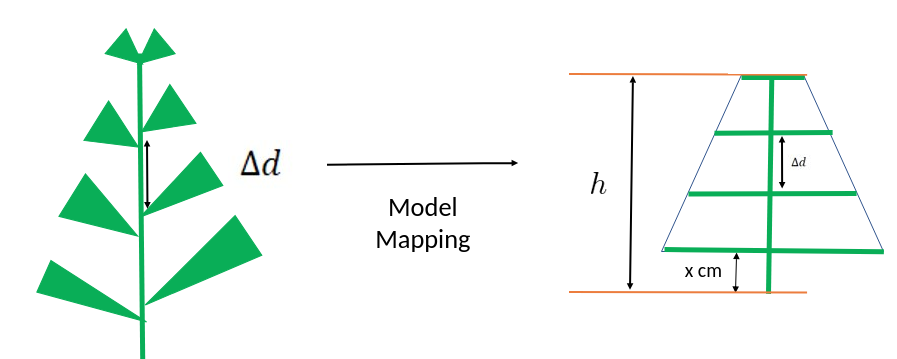
\includegraphics[width=0.9\textwidth,height=\textheight,keepaspectratio]{modelling/plant-model-3.png}
    \caption{Tomato plant model}
    \label{fig:plant:model:2}
\end{figure}

This model especially serves for the purpose of LAI calculation where the canopy visible from above can 
be mapped to the largest (and lowest) branch level of the plant - whereby each higher (and therefore newer)
level is smaller.
The size of the plant's entire leaf area is then correlated with the number of levels.
This model will be formalized in more detail later with all of its parameters. 

\subsection{Computational Pipelines}
\input{members/ssr/authors}

To estimate the central LAI metric, two computation pipelines are combined to extract specific metrics from images.
Each pipeline applies a series of image processing and computations in order to contribute to the result
in the following ways:

\begin{enumerate}
    \item \textbf{Pipeline A:} Estimates the \textit{leaf area} (not LAI) which is the visible canopy
    of a single plant, captured by camera mounted above of the plants.
    \item \textbf{Pipeline B:} Estimates the plant height, based on an image taken from a different camera,
    with a specific setup.
\end{enumerate}

Both metrics are then combined (with additional statistical corrections) to estimate the actual LAI.
Again, the LAI is different from the \textit{leaf area} in the way that it contains
the \textit{entire} existing leaf area and not only the leaf area which is visible from above.

\subsection{Pipeline A}\label{subsec:pipeline-a}

Introduce ...

\begin{figure}[H]
    \centering
    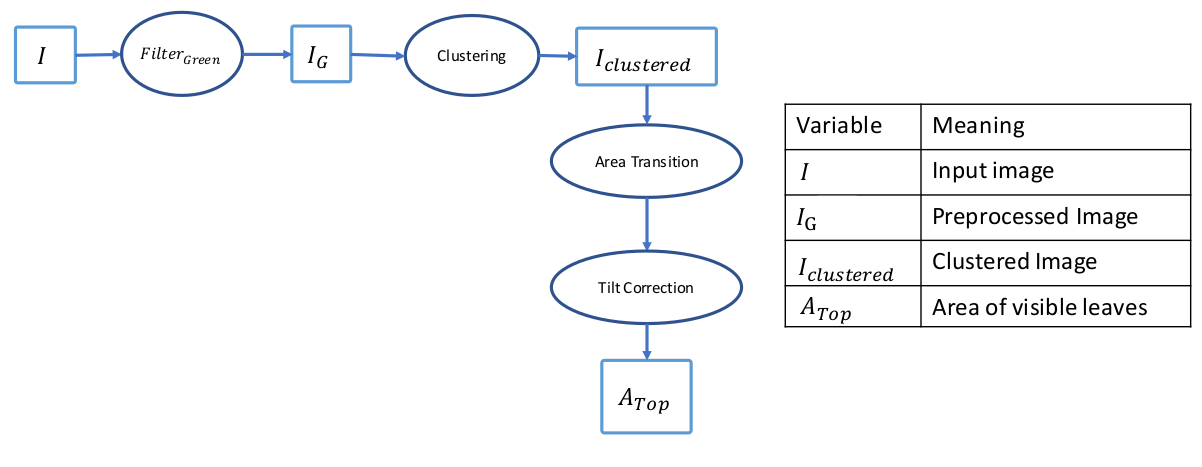
\includegraphics[width=1.0\textwidth]{modelling/pipeline-a.png}
    \caption{The pipeline can be accessed by web browser or purely on a Windows desktop.}
    \label{fig:p:a}
\end{figure}

\graphicspath{{members/ssr/figures/}}

\subsubsection{Camera Setup}
\input{members/ssr/authors}

The input data for Pipeline A is acquired through a digital photo camera which is mounted above the
plants and can move along each lane and take an image from every single plant.
Each captured image contains a square of a ground unit which shows only one plant from above
showing it's canopy, as shown in figure \ref{fig:pipeline:a:camera:setup}

\begin{figure}[H]
    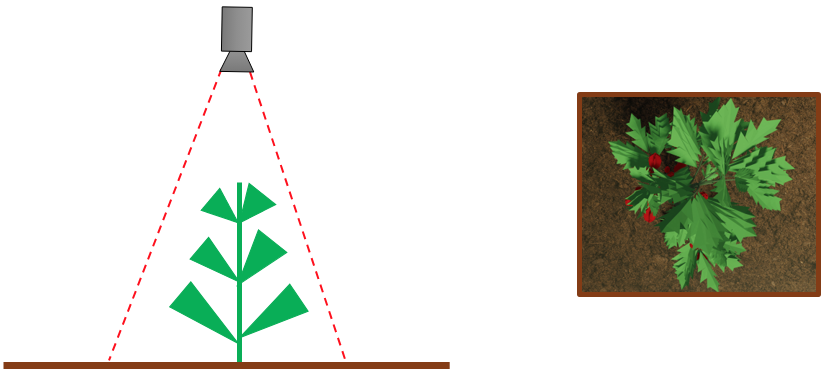
\includegraphics[width=0.9\textwidth,height=\textheight,keepaspectratio]{modelling/camera-setup.png}
    \caption{Camera setup for input data for Pipeline A. Right: Canopy image taken by the camera}
    \label{fig:pipeline:a:camera:setup}
\end{figure}

This basic metric is fed into the pipeline for further processing.
Its purpose is to measure the canopy size which is done by segmentation, as presented in the next chapter.
\subsubsection{Leaf Area Segmentation}\label{subsec:segmentation}
\input{members/ssr/authors}

\textit{Segmentation} here refers to the process of \textit{image segmentation}, which is the process
of partitioning an image into multiple areas or segments which have distinct meanings.\\

In this specific context, the purpose of the segmentation it to distinguish the canopy of one plant
from it's surrounding.

The specific greenhouse layout allows to assume that crops are planted in lanes, next to each other, this
allows to take individual images from above only showing the canopy.

If this constrain is not met, then the presented approach will break, since one plant can't be
differentially from another.

Since individual plants are capture per image the green color dominating areas must belong to the
plant's canopy, hence a simple approach to segmentation can be used by finding all pixel with
dominating green color ratio, which is the case when following condition is true:

\[
    \frac{G + \epsilon}{\max{\{R, B\}} + \epsilon} > 1.0 
\]\\

Where $R, G, B$ are values of each color channels of each pixel, with small $\epsilon$ to prevent division by zero.
High red values indicate either dry leaves or red tomatoes - which are both not part of the leaf
area.
Green tomatoes are also irrelevant since they lie on top of leaves and branches and don't increase
accidentally the leaf area.\\

Once the canopy of a plant can be separated from it's surrounding then the proportion of visible leaf
area from above can be calculated per ground unit which is visible on the image.
The segmented leaf area can then be measured and mapped to the model as illustrated
by figure \ref{fig:mapping}

\begin{figure}[H]
    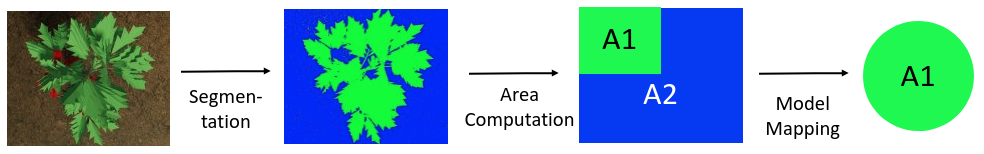
\includegraphics[width=\textwidth,height=\textheight,keepaspectratio]{modelling/mapping.png}
    \caption{Mapping the visible leaf area to lowest level of plant model}
    \label{fig:mapping}
\end{figure}

Once the canopy size is estimated, it can be used in later stages to map it to the plant model.
Figure \ref{fig:canopy} shows the relation between canopy and model mapping.

\begin{figure}[H]
    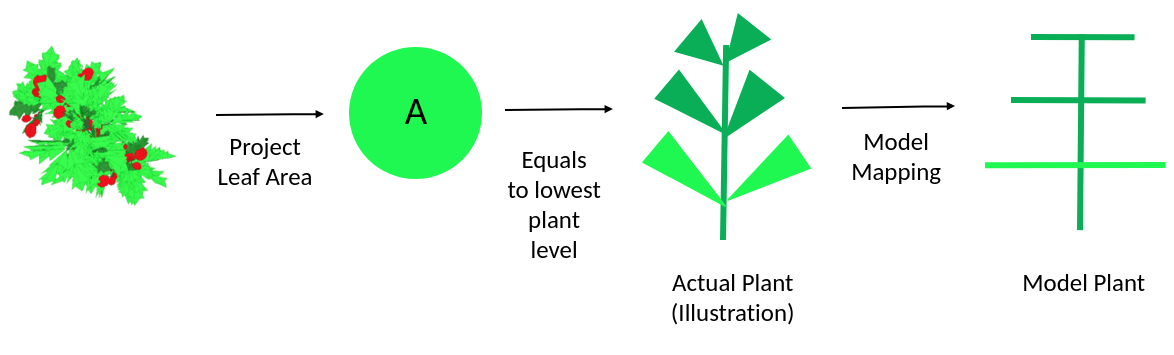
\includegraphics[width=\textwidth,height=\textheight,keepaspectratio]{modelling/plant-model.png}
    \caption{Mapping canopy to plant model}
    \label{fig:canopy}
\end{figure}

As it is obvious, this assumes that the lowest level is the biggest visible area from above
and the number of levels and the size of each level still needs to be estimating for estimating the
entire leaf area.
This will be described in later sections more formally.

